\chapter{Results}
REPLACE WITH ACTUAL CONTENTS.

\section{Section 1}

\begin{table}[h]
\centering
\begin{tabular}{|l|l|l|l|}
\hline
         & Scissors & Paper & Stone \\ \hline
Scissors & Draw     & Win   & Lose  \\ \hline
Paper    & Lose     & Draw  & Win   \\ \hline
Stone    & Win      & Lose  & Draw  \\ \hline
\end{tabular}
\caption{Rules for Scissors-Paper-Stone.}
\label{table:example}
\end{table}

Table~\ref{table:example} shows an example table.

\section{Section 2}

\begin{figure}[h]
\centering
\begin{subfigure}[b]{.5\textwidth}
  \centering
  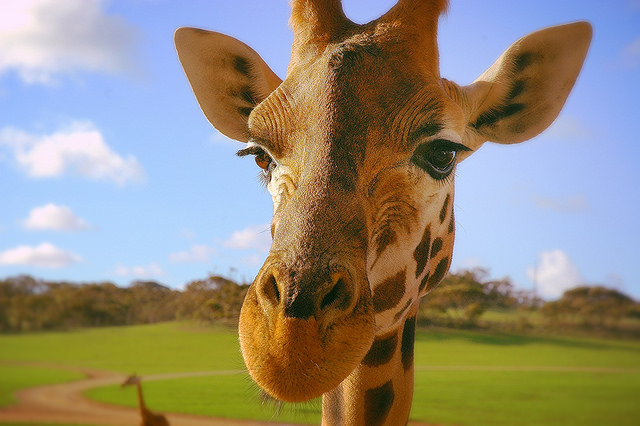
\includegraphics[width=.5\linewidth]{giraffe.jpg}
  \caption{An adorable Giraffe.}
\end{subfigure}%
\begin{subfigure}[b]{.5\textwidth}
  \centering
  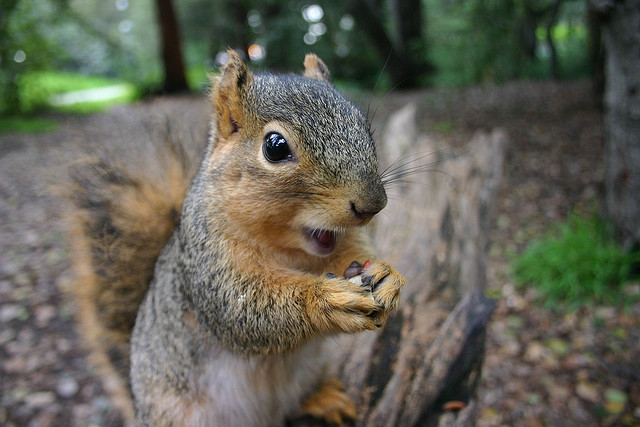
\includegraphics[width=.5\linewidth]{squirrel.jpg}
  \caption{An adorable Squirrel.}
\end{subfigure}
\caption{Adorable Animals.\label{fig:example}}
\end{figure}

In Figure~\ref{fig:example}, we have an example of images as sub-figures. Also animals.